\documentclass{beamer}
\usetheme{Dresden}
%\usetheme{CambridgeUS}
\usepackage{helvet}
\usepackage{cite}
\usepackage{url}
\usepackage{amssymb, amsmath, graphicx, charter, latexsym}
\usepackage{subfigure}
\usepackage{enumerate}
\usepackage{ragged2e}
\usepackage{mathtools}
\usepackage{tabu}
\usepackage{epstopdf}
\usepackage{siunitx}
\usepackage{calligra}
\usepackage{listings}
\usepackage{todonotes}
\renewcommand{\familydefault}{\sfdefault}
%\usepackage{times}

\setbeamertemplate{items}[circle]
\setbeamertemplate{navigation symbols}{}
\setbeamertemplate{caption}{\insertcaption}

\newcommand{\argmax}{\operatorname{argmax}}
\lstset{
basicstyle=\ttfamily,
}

\begin{document}
\title{S-WiFi: Smart Scheduling for WiFi Uplink Transmissions with Point Coordination Function}
\author{Dongni Han, Ping-Chun Hsieh, and Tao Zhao}
\date{April 28, 2016}
\newtheorem{thm}{Theorem}
\begin{frame}
\titlepage
\end{frame}


%\begin{frame}
%\frametitle{What to Discuss Today?}
%\tableofcontents[]
%\end{frame}

%\AtBeginSection[]
%{
	%\begin{frame}{Table of Contents}
	%\tableofcontents[currentsection]
	%\end{frame}
%}

\NewDocumentCommand{\varSI}{O{}}{\SI[detect-all=true,parse-numbers=false,#1]}

\section{Background}

\begin{frame}
\frametitle{System Model}
\begin{itemize}
  \item WiFi network
    \begin{itemize}
      \item One AP and $N$ clients
      % \varSI must be outside math env for it to have right font family.
      \item Time slotted; $\SI{1}{interval} =$ \varSI{T}{slots}
    \end{itemize}
  \item Uplink Transmissions
    \begin{itemize}
      \item Packets generated at each client $n$ in each interval $k$
      \item Number of packets $X_n$ follows Unif$\{U_\text{min}, U_\text{max}\}$
      \item Real-time traffic
    \end{itemize}
  \item Point Coordination Function (PCF)
    \begin{itemize}
      \item AP polls (at most) one client per slot
      \item But AP needs to know $X_n$ first!
    \end{itemize}
\end{itemize}
\end{frame}

\begin{frame}
\frametitle{Baseline Policy: Phase 1}
\begin{itemize}
\item AP polls $X_n$ for all $n$ one by one
\end{itemize}
\begin{figure}
\centering
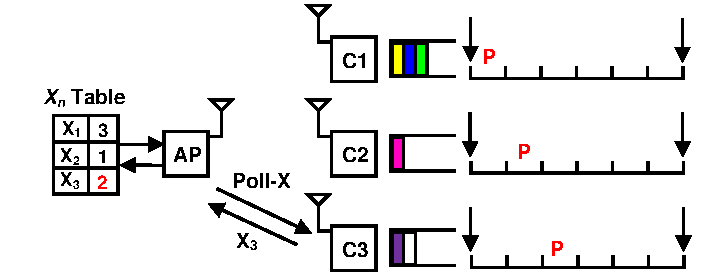
\includegraphics[scale=0.8]{animation_03.pdf}
\end{figure}
\end{frame}

\begin{frame}
\frametitle{Baseline Policy: Phase 2}
\begin{itemize}
\item AP uses Max-Weight scheduling for data transmissions
\end{itemize}
\begin{figure}
\centering
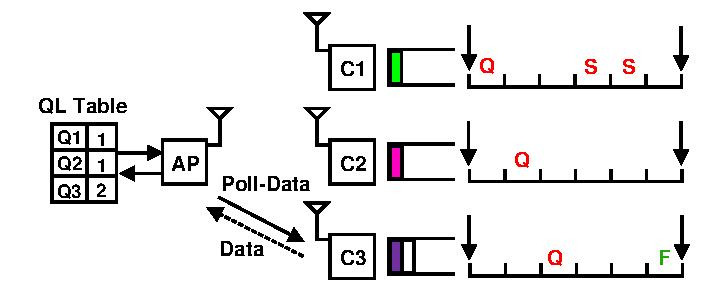
\includegraphics[scale=0.8]{animation_06.pdf}
\end{figure}
\end{frame}

\begin{frame}{Baseline Policy: Issues}
  \begin{itemize}
    \item No data transmissions in Phase 1
    \item Channel utilization for data packets is low
    \item Huge overhead especially with large $N$ and bad channels
      \pause
    \item We need a smart policy!
  \end{itemize}
\end{frame}
\section{Smart Policy}

\begin{frame}
\frametitle{Idea 1: Selective Polling}
\begin{itemize}
\item Only poll $n \le N$ clients per interval
\item Random permutation for fairness and stability
\item Schedule remaining clients only after all selected are scheduled
\end{itemize}
\begin{figure}
\centering
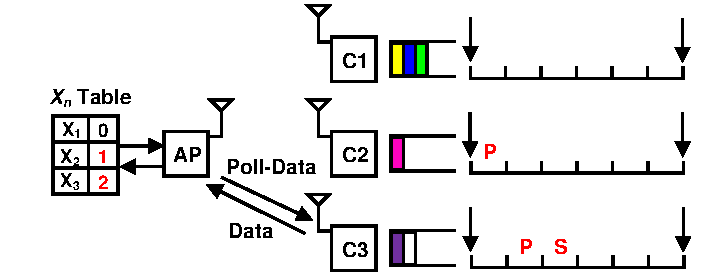
\includegraphics[scale=0.8]{selective_1.pdf}
\caption{Example: $n=2, N=3$}
\end{figure}
\end{frame}

\begin{frame}
\frametitle{Feature 001: Selective Polling}
\begin{itemize}
\item How to determine the optimal $n$?
  \begin{itemize}
    \item Sort clients by channel reliabilities $p_1 > p_2 > \dots > p_N$
    \item Estimated throughput: $\hat{R}_n = \min\{n, (T-\sum_{i=1}^{n}\frac{1}{p_i})\frac{\sum_{i=1}^{n}p_i}{n} \}$
    \item Find the optimum $n^* = \argmax_{n} \hat{R}_n$
  \end{itemize}
\item Random permutation?
  \begin{itemize}
    \item Classic problem: Knuth shuffle algorithm
  \end{itemize}
\item How to schedule remaining clients?
  \begin{itemize}
    \item Greedy: poll $X_n$ and data one by one
  \end{itemize}
\end{itemize}
\end{frame}

\begin{frame}
\frametitle{Idea 2: Piggybacked Queue Length}
\begin{itemize}
\item Client replies in one packet
  \begin{itemize}
    \item $X_n$
    \item first data message if $X_n>0$
  \end{itemize}
\end{itemize}
\begin{figure}
\centering
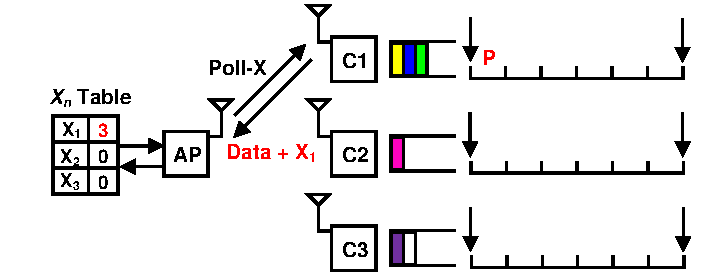
\includegraphics[scale=0.8]{piggyback_1.pdf}
\end{figure}
\end{frame}

\begin{frame}
\frametitle{Feature 010: Piggybacking}
\begin{itemize}
  \item New packet types
    \begin{itemize}
      \item \lstinline|SWiFi_PKT_POLL_PGBK|
      \item \lstinline|SWiFi_PKT_PGBK_UL|
    \end{itemize}
  \item If combined with selective polling
    \begin{itemize}
      \item All slots are effectively available for data
      \item Estimated throughput: $\hat{R}_n = \min\{n, \alert{T}\frac{\sum_{i=1}^{n}p_i}{n} \}$
    \end{itemize}
\end{itemize}
\end{frame}

\begin{frame}
\frametitle{Idea 3: Retry Limit for Polling}
\begin{itemize}
\item Avoid spending too much time on clients with poor channel
\end{itemize}
\begin{figure}
\centering
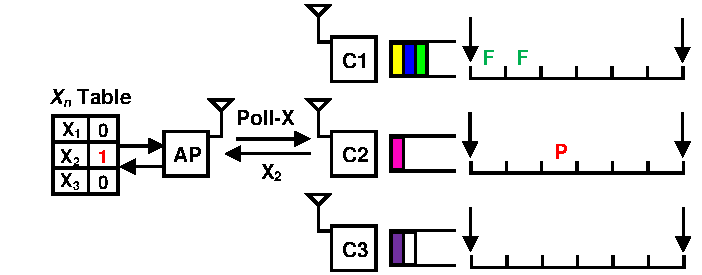
\includegraphics[scale=0.8]{retry_1.pdf}
\caption{Example: $p_1=0.1$, retry limit $= 1$}
\end{figure}
\end{frame}

\begin{frame}
\frametitle{Feature 100: Retry Limit}
\begin{itemize}
  \item Set \lstinline|num_retry_ = 0| for the newly polled client
  \item If retry limit reached: poll the next client in the next interval
    no matter the last transmission is successful or not
  \item Otherwise: \lstinline|num_retry_++|
\end{itemize}
\end{frame}

\begin{frame}{Feature 111: Our Smart Policy}
  \begin{itemize}
    \item Selective Polling + Piggybacking + Retry Limit
      \begin{itemize}
	\item Selective a subset of clients to poll $X_n$
	\item AP polls clients in expect of piggybacking reply
	\item AP repeats polling a client for limited times
      \end{itemize}
    \item All combinations of three features are possible
      \begin{itemize}
	\item Special case: baseline $=$ 000
      \end{itemize}
  \end{itemize}
\end{frame}

\section{Simulation}
\begin{frame}{Simulation Setup}
  \begin{itemize}
    \item $\SI{1}{slot} = \SI{10}{ms}, T=10$
    \item Number of clients $N=5$
    \item Number of packets $U_\text{min}=0, U_\text{max}=2$
    \item Channel
      \begin{itemize}
	\item Symmetric: $p_i=p, i=1,2,\dotsc,N$
	\item Asymmetric: $p_1=p_2=1;\quad p_i=p, i=3,4,\dotsc,N$
	\item $p\approx0.57$ (distance \SI{1000}{m})
      \end{itemize}
    \item Metric: total timely-throughput of all clients
      \begin{itemize}
	\item Averaged over 10 runs
      \end{itemize}
  \end{itemize}
\end{frame}
%\begin{frame}
%\frametitle{Simulation Results: Network Capacity}
%\begin{itemize}
%\item $N=2$ and $T=10$
%\item Reliable channel: $p_1 = p_2 = 1$ (symmetric)
%\item $N_\text{max}$ ranges from $1$ to $20$
%\item Real-time traffic
%\end{itemize}
%\begin{figure}
%\centering
%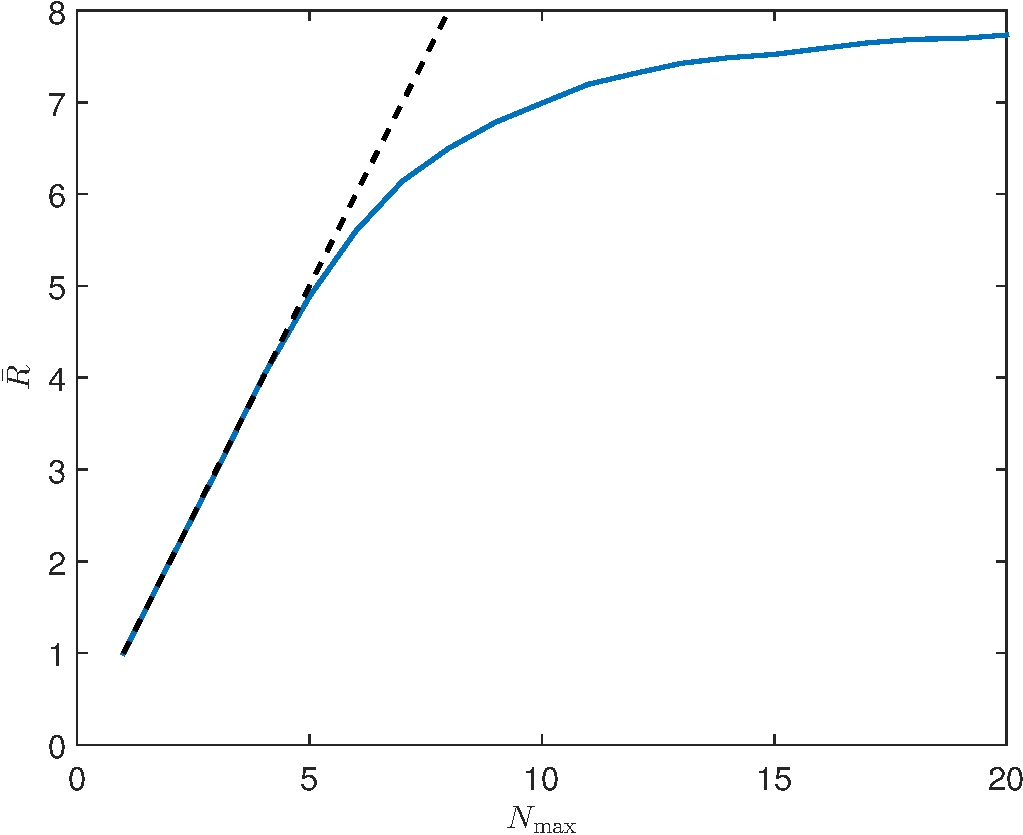
\includegraphics[height=.5\textheight]{realtime_throughput_randmax.pdf}
%\caption{Packet deadline reduces the capacity further.}
%\end{figure}
%\end{frame}

\begin{frame}
\frametitle{Performance under Symmetric Channel}
\begin{itemize}
\item $p$ ranges from $0$ to $1$
\end{itemize}
\begin{figure}[htbp]
  \centering
  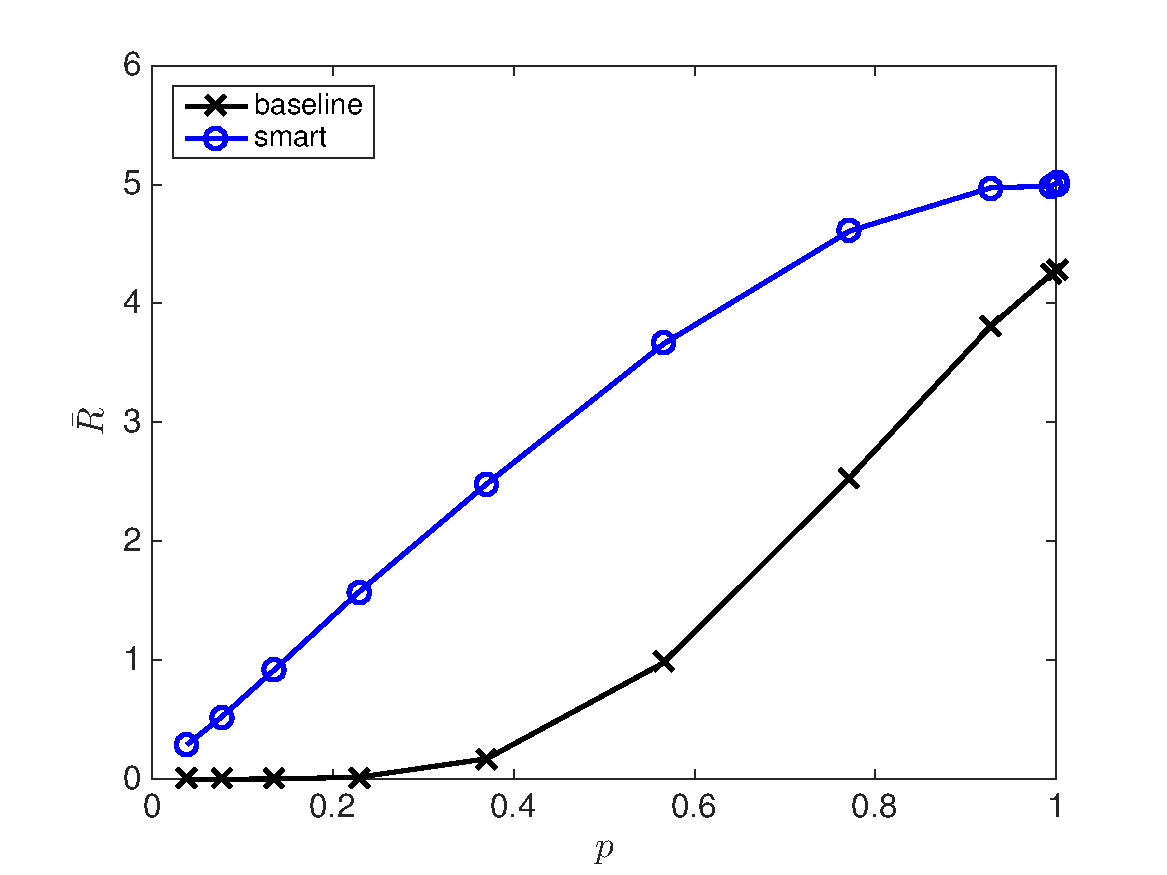
\includegraphics[height=.5\textheight]{R_p_sym.pdf}
  \caption{Throughout v.s. channel reliability.}
\end{figure}
\end{frame}

\begin{frame}
\frametitle{Performance under Asymmetric Channel}
\begin{itemize}
\item $p$ ranges from $0$ to $1$
\end{itemize}
\begin{figure}[htbp]
  \centering
  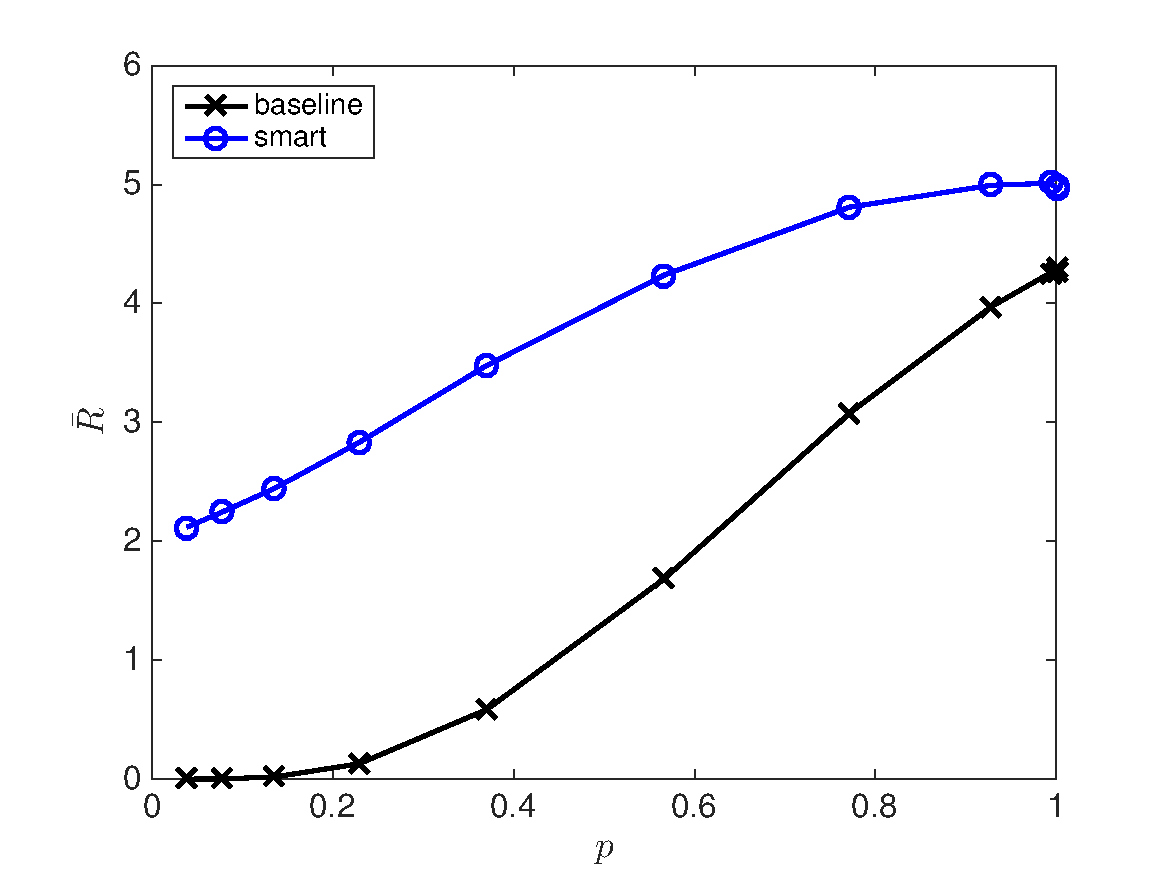
\includegraphics[height=.5\textheight]{R_p_asym.pdf}
  \caption{Throughout v.s. channel reliability of distant clients.}
\end{figure}
\end{frame}

\begin{frame}
\frametitle{Impact of Number of Packets}
\begin{itemize}
  \item $U_\text{max}$ ranges from $2$ to $10$ FIXME
  \item $U_\text{min}=0$ FIXME
  \item Symmetric channel FIXME
\end{itemize}
\begin{figure}[htbp]
  \centering
  %\includegraphics[height=.5\textheight]{R_U.pdf}
  \missingfigure{Testing a long text string}
  \caption{Throughout v.s. number of packets.}
\end{figure}
\end{frame}

\begin{frame}
\frametitle{Impact of Number of Clients}
\begin{itemize}
\item $N$ ranges from $1$ to $10$ FIXME
\item Symmetric channel FIXME
\end{itemize}
\begin{figure}[htbp]
  \centering
  %\includegraphics[height=.5\textheight]{R_N.pdf}
  \missingfigure{Testing a long text string}
  \caption{Throughout v.s. number of clients.}
\end{figure}
\end{frame}

\begin{frame}{Network Utility}
  \begin{itemize}
    \item $q_n$: timely-throughput for client $n$
    \item $U_n(q_n) = \log (100 q_n)$
  \end{itemize}
\begin{figure}[htbp]
  \centering
  %\includegraphics[height=.5\textheight]{R_N.pdf}
  \missingfigure{Testing a long text string}
  \caption{Network utility v.s. channel reliability.}
\end{figure}
\end{frame}

\begin{frame}{Fairness}
\begin{figure}[htbp]
  \centering
  %\includegraphics[height=.5\textheight]{R_N.pdf}
  \missingfigure{Testing a long text string}
  \caption{Utility of each clients.}
\end{figure}
\end{frame}

\section*{Conclusion}
\begin{frame}{Conclusion}
  \begin{itemize}
    \item The baseline policy incurs huge overhead especially with large $N$ and bad channel.
    \item Our smart policy incoporates selective polling, piggybacking, and
      retry limit to improve the performance.
    \item Simulation shows our smart policy outperforms the baseline policy in
      terms of timely-throughput, network utility, and fairness.
  \end{itemize}
\end{frame}

\begin{frame}{Outlook}
  \begin{itemize}
    \item Selective: non-uniform permutation
    \item Piggybacking: non-real-time traffic
    \item Retry limit: optimum
    \item Phase 2: Debt based policies
    \item S-WiFi logo, website, etc.
  \end{itemize}
\end{frame}

\begin{frame}
  \begin{center}
    {\Huge\calligra Thank you!}
  \end{center}
  \begin{figure}[htbp]
    \centering
    
\includegraphics[height=.3\textheight]{url.pdf}
  \end{figure}
\end{frame}
\end{document}
